\section{Schemat drabinkowy w programie LOGO!Soft Comfort}
\label{sec:drabinka}

\subsection{Zasady odwzorowania}
Równania z punktów~\ref{sec:zdarzenia} i~\ref{sec:rownania} zostały
odwzorowane w języku drabinkowym LAD
(zob.~\cite{legierski,flaga}) z użyciem bloków sterownika LOGO!
\cite{logo}. Przyjęto następujące zasady:
\begin{itemize}
    \item styki połączone szeregowo w jednym rzędzie realizują
          iloczyn logiczny (AND),
    \item rzędy łączone przewodami w jednym wejściu bloku realizują
          sumę logiczną (OR) -- np. dwa rzędy podłączone do wejścia $S$
          bloku RS,
    \item styk normalnie otwarty (NO) odpowiada zmiennej $A$,
          a normalnie zamknięty (NC) zmiennej $\overline{A}$,
    \item stan przerzutników RS jest odczytywany stykiem typu
          ,,wyjście bloku'' i przepisywany do markera cewką,
    \item wszystkie bloki mają parametr \texttt{Rem=off}, więc po
          restarcie programu układ startuje w stanie $S_0$.
\end{itemize}
Zastosowane bloki zestawiono w tabeli~\ref{tab:bloki}.

\begin{table}[H]
\centering
\caption{Bloki programu w LOGO!Soft Comfort.}
\label{tab:bloki}
\begin{tabular}{lll}
\toprule
Oznaczenie & Typ bloku & Parametry \\
\midrule
$T_{001}$ & opóźnienie załączania (TON) & \SI{0,50}{\second}, \texttt{Rem=off} \\
$T_{002}$ & opóźnienie załączania (TON) & \SI{2,00}{\second}, \texttt{Rem=off} \\
RS\_M2 (SF003) & przerzutnik RS & \texttt{Rem=off} \\
RS\_M3 (SF004) & przerzutnik RS & \texttt{Rem=off} \\
RS\_M1 (SF005) & przerzutnik RS & \texttt{Rem=off} \\
\bottomrule
\end{tabular}
\end{table}

\subsection{Kolejność sieci}
W sterowniku sieci są wykonywane kolejno od góry do dołu, a marker
odczytany przed zapisem ma wartość z poprzedniego cyklu. Poprawne
działanie programu zależy od tej kolejności:
\begin{itemize}
    \item sieć~7, zapisująca $M_7$, $M_8$, $M_9$, musi być ostatnia --
          w przeciwnym razie zdarzenia przestałyby być jednocyklowe,
    \item sieć~3 (ekran) musi poprzedzać sieć~4 (menu), a obie
          sieć~5 (telefon). Dzięki temu w cyklu zdarzenia sieci~3 i~4
          widzą jeszcze poprzednie wartości $M_3$ i $M_1$,
          zgodnie z równaniami~\eqref{eq:s2}--\eqref{eq:r3}.
\end{itemize}

\subsection{Sieć 1 -- pomiar czasu}
Sygnał $I_1$ pobudza oba timery TON (rys.~\ref{fig:siec1}). Wyjście
$T_{001}$ jest aktywne po \SI{0,5}{\second} trzymania przycisku,
a $T_{002}$ po \SI{2}{\second}.

\begin{figure}[H]
\centering
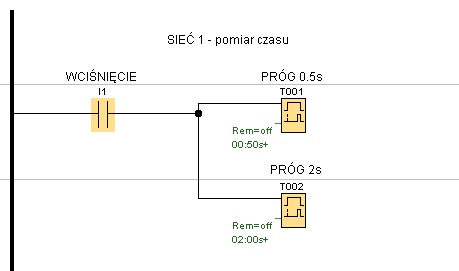
\includegraphics[width=0.6\textwidth]{rys/siec_1.png}
\caption{Sieć 1 -- pomiar czasu przytrzymania przycisku.}
\label{fig:siec1}
\end{figure}

\subsection{Sieć 2 -- rozpoznawanie kliknięć}
Sieć~2 (rys.~\ref{fig:siec2}) realizuje równania~\eqref{eq:k},
\eqref{eq:s} i~\eqref{eq:d}. Cewki $M_4$, $M_5$ i $M_6$ są aktywne
przez jeden cykl programu.

\begin{figure}[H]
\centering
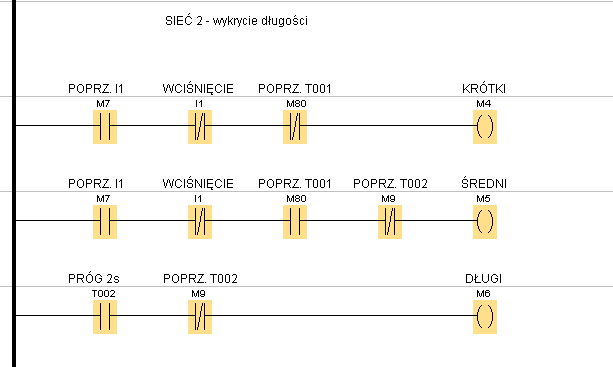
\includegraphics[width=0.85\textwidth]{rys/siec_2.png}
\caption{Sieć 2 -- wykrycie długości kliknięcia (zdarzenia K, Ś, D).}
\label{fig:siec2}
\end{figure}

\subsection{Sieć 3 -- stan ekranu}
Przerzutnik RS\_M2 realizuje równania~\eqref{eq:s2} i~\eqref{eq:r2}
(rys.~\ref{fig:siec3}). Do wejścia $S$ prowadzą dwa rzędy:
$M_4\,M_1\,\overline{M_3}\,\overline{M_2}$ oraz
$M_6\,\overline{M_1}$. Do wejścia $R$ prowadzą dwa rzędy:
$M_4\,M_1\,\overline{M_3}\,M_2$ oraz $M_6\,M_1$. Wyjście
przerzutnika jest przepisywane cewką do markera $M_2$.

% TODO: po poprawce rzedu 2 (M6 * /M1 zamiast M6 * /I1) wykonac nowy
% zrzut ekranu i podmienic rys/siec_3.png.
\begin{figure}[H]
\centering
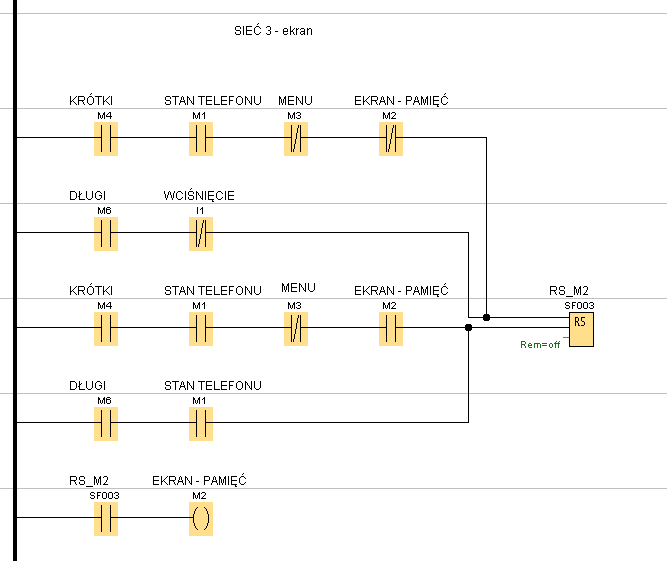
\includegraphics[width=0.85\textwidth]{rys/siec_3.png}
\caption{Sieć 3 -- sterowanie stanem ekranu (przerzutnik RS\_M2).}
\label{fig:siec3}
\end{figure}

\subsection{Sieć 4 -- menu wyłączenia}
Przerzutnik RS\_M3 realizuje równania~\eqref{eq:s3} i~\eqref{eq:r3}
(rys.~\ref{fig:siec4}). Wejście $S$ jest wysterowane rzędem
$M_5\,M_1$, a wejście $R$ sumą dwóch rzędów: $M_4\,M_3$ oraz $M_6$.

\begin{figure}[H]
\centering
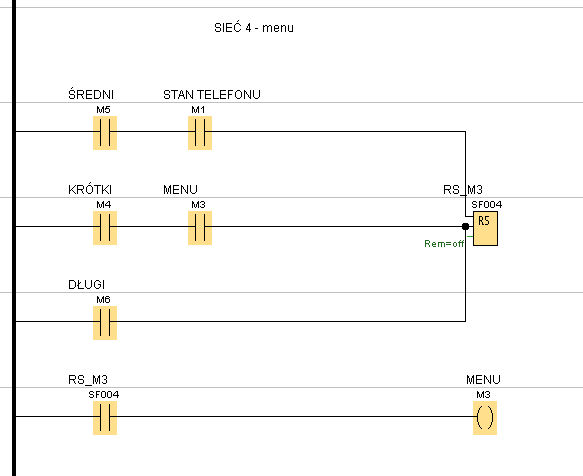
\includegraphics[width=0.8\textwidth]{rys/siec_4.png}
\caption{Sieć 4 -- sterowanie menu wyłączenia (przerzutnik RS\_M3).}
\label{fig:siec4}
\end{figure}

\subsection{Sieć 5 -- stan telefonu}
Przerzutnik RS\_M1 realizuje równania~\eqref{eq:s1} i~\eqref{eq:r1}
(rys.~\ref{fig:siec5}). Ponieważ zdarzenie $M_6$ trwa jeden cykl,
każde kliknięcie D zmienia stan telefonu dokładnie raz.

\begin{figure}[H]
\centering
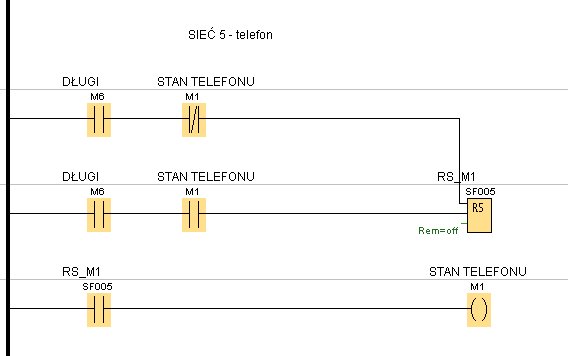
\includegraphics[width=0.8\textwidth]{rys/siec_5.png}
\caption{Sieć 5 -- sterowanie stanem telefonu (przerzutnik RS\_M1).}
\label{fig:siec5}
\end{figure}

\subsection{Sieć 6 -- wyjścia}
Wyjścia układu odwzorowują równania~\eqref{eq:q2} i~\eqref{eq:q1}
(rys.~\ref{fig:siec6}). Równoległe połączenie styków $M_2$ i $M_3$
realizuje sumę $M_2 + M_3$, a szeregowy styk $M_1$ -- iloczyn
z tą sumą.

\begin{figure}[H]
\centering
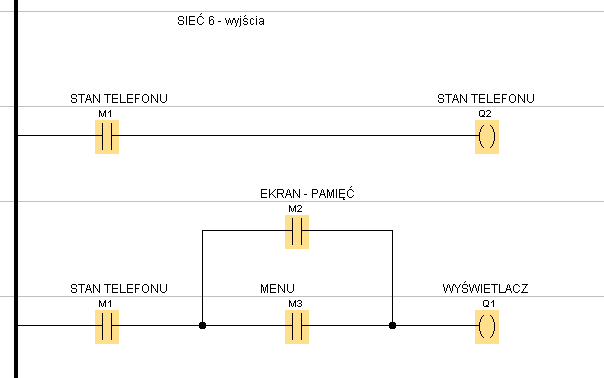
\includegraphics[width=0.8\textwidth]{rys/siec_6.png}
\caption{Sieć 6 -- sterowanie wyjściami $Q_1$ i $Q_2$.}
\label{fig:siec6}
\end{figure}

\subsection{Sieć 7 -- pamięć poprzedniego cyklu}
Ostatnia sieć programu (rys.~\ref{fig:siec7}) zapisuje wartości
$I_1$, $T_{001}$ i $T_{002}$ w markerach $M_7$, $M_8$ i $M_9$
(równanie~\eqref{eq:poprzedni}).

\begin{figure}[H]
\centering
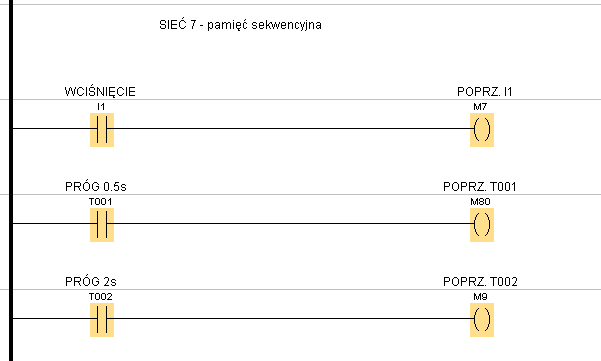
\includegraphics[width=0.8\textwidth]{rys/siec_7.png}
\caption{Sieć 7 -- pamięć poprzedniego cyklu programu.}
\label{fig:siec7}
\end{figure}
